\chapter{State of the Art}
\label{State of the Art}
\thispagestyle{empty}


In this chapter we will explain basic concepts and theoretical background needed to the understanding of our work and that our work is based on. In particular, we give the notion of what is a learning agent, what are its key features and what are the other building blocks that compose the Reinforcement Learning framework. Then, we describe the main algorithms used to solve a Markov Decision Process and their extension to practical problems such as autonomous driving, videogames and in particular racing games.

\section{Theoretical Background}

\subsection{Reinforcement Learning Background}
\begin{figure}[t]
 \centering
  \captionsetup{width=10cm}
  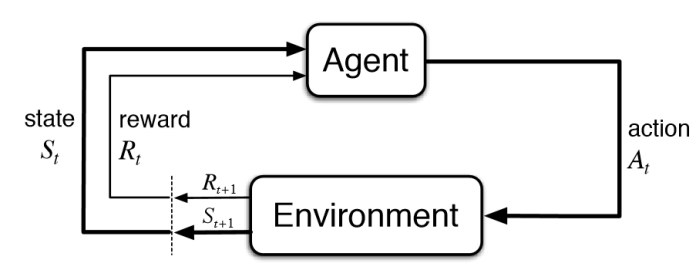
\includegraphics[width=10cm]{./img/rl}
  \caption{The basic RL loop. An agent in a state $s_t$ takes an action $a_t$ in an environment, which takes it in a state $s_{t+1}$ and receives a reward accordingly.}
   \label{fig:rl-loop}
\end{figure}
Together with Supervised Learning and Unsupervised Learning \cite{elements}, Reinforcement Learning (RL) is a branch of Machine Learning, the discipline which studies the way a computer program can learn from experience and improve its performance at a specified task. Whereas Supervised Learning algorithms are based on inductive inference where the model is typically trained using labelled data to perform classification or regression, and Unsupervised Learning exploits techniques of density estimation and clustering applied to unlabelled data, in the Reinforcement Learning paradigm an autonomous agent learns what to do (how to map situations to actions) so as to maximize a numerical reward signal by interacting with the environment.

Typically, the RL agent is not explicitly taught how to act by an expert, but it must discover which action yields the largest reward in a trial-and-error procedure, the so called exploration phase. As the learner gathers experience it becomes able to distinguish good actions from bad actions and therefore it can exploit its knowledge to reach the goal of maximizing the reward signal received at each step of the interaction.
The challenge of Reinforcement Learning is to design the best trade-off between exploration and exploitation, that is the capability of an agent to use its knowledge to obtain high rewards and, by contrast, being capable of exploring new possibilities in such a way not to remain stuck in a local optimum. Intuitively, the exploration process is high at the first iterations of the learning process, while it should decrease with accumulating knowledge.

\subsubsection{Markov Decision Process}
An RL setting is composed by an \textit{agent}, that is the learner and the decision maker, which interacts with an \textit{environment}. The environment is the mathematical representation of the world in which the agent operates. It reflects the set of features of a machine learning problem, which could be numerical (coordinates, velocities, acceleration) or raw (such as images or signals). The choice of the algorithm suitable to perform a learning process depends on the representation of the environment. At each time step $t$, the agent receives a representation of the environment's \textit{state} $S_t \in S$, based on which it selects an \textit{action} $A_t \in A$ to perform. In the following time step $t+1$, the agent receives a numerical reward $R_{t+1} \in R \in \mathbb{R}$ based on the goodness of its decision. Then, it gets in a new state $S_{t+1}$ (see Figure~\ref{fig:rl-loop}). The sequence of states and actions is called $trajectory$.

The RL setting can be formalized as a Markov Decision Process. An MDP is a tuple $<S,A,p,R>$ composed by:
\begin{itemize}
  \item A set of states \(S\): it encompasses every possible state of the process;
  \item A set of actions \(A\): it represents the possible action the agent can take at any moment;
 \item A transition probability function \(p(S_{t+1} = s',R_{t+1} = r|S_t=s, A_t=a) \), which indicates the probability of landing in a state \(s'\) being in a state \(s\) taking an action \(a\) and taking a reward $r$.
 \item A reward function \(R(s, a) = \mathbb{E}[R_t|S_{t-1}=s, A_{t-1}=a]\), the reward received after transitioning from state $s$ to state $s$', due to action $a$. This is true only if the transition probability function does not include the reward itself.

\end{itemize}
$R_t$ and $S_t$ are random variables with probability distributions dependent only on the preceding state and action. That is, for particular values of these random variables, $s' \in S$ and $r \in  R$, there is a probability of those values occurring at time $t$, given particular values of the preceding state and action. 
In a Markov decision process, the probabilities given by $p$ completely characterize the
environment’s dynamics. That is, the probability of each possible value for $S_t$ and $R_t$
depends only on the immediately preceding state and action $S_{t-1}$ and $A_{t-1}$. This is called the \textit{Markov property}.

An finite MDP (an MDP with finite set of states and finite set of actions) can be solved through Dynamic Programming \cite{irl}. However, in real-world scenarios, typically we do not have full knowledge of the MDP, or it is too complex to solve through such methods. In such cases, RL can be used. By contrast, when the dynamics is not known apriori, i.e.  transition model is unknown, or it is too complex, i.e. there are too many state to consider, RL can be used, which operates by receiving only samples of the process. 

\subsubsection{Return}
At each time step, the agent receives a reward for the taken action by the environment as a number,  $R_t \in \mathbb{R}$ in a specific state. The agent's goal is to maximize the expected value of the cumulative sum of a received reward $G_t$, called \textit{expected return}, where the return is a function of the reward sequence:\begin{equation}G_t = \sum^{\infty}_{k=0}\gamma^k r_{t + k +1},\label{eqn:return}\end{equation}
where $\gamma$ is  parameter, \(0 \leq \gamma \leq 1\), called \textit{discount factor}. The discount factor influences how the agent considers future and present rewards. A small \(\gamma\) results in a higher consideration of present rewards than the future, leading to a "myopic" maximization of reward, while with a \(\gamma\) near to 1, the agent will consider equally the reward coming from the present either from the future, becoming more "farsighted". According to the the nature of the problem, the task can be \textit{episodic} or \textit{continuous}. In the former case, the learning process is subdivided in \textit{episodes}, all of which terminate with a \textit{terminal state} at time $T$, where $T$ is a stochastic variable. In the latter, by contrast, there is no terminal state, but the learning process can go on indefinitely. Thus, the expected return $G_t$ is changed by adding a discount factor that avoids $G_t$ to diverge to infinity.


\subsubsection{Policies and Value Functions}
The goal of reinforcement learning is finding a policy \(\pi\), which maps states to a probability distribution over the actions, in order to maximize the return. If the agent is following policy $\pi$ at time $t$, then $\pi(a|s)$ is the probability that $A_t = a$ if $S_t = s$. 

The \textit{value function} of a state $s$ under a policy $\pi$, denoted $v_\pi(s)$ is defined as the expected long-term return starting from the current state under policy $\pi$: 
\begin{equation}
v_\pi(s) = \mathbb{E}_\pi{\left[G_t|S_t=s\right]}= \mathbb{E}_\pi\left[\sum^{\infty}_{k=0}\gamma^k R_{t+k+1}|S_t=s\right] , \label{eqn:value}
\end{equation} for all $s \in \mathcal{S}$, where $E_\pi[\cdot]$ denotes the expected value of a random variable given that the agent follows policy $\pi$.
The \textit{action-value function} for a policy $\pi$ is defined as the value of taking action $a$ in a state $s$ and following $\pi$:
\begin{equation} q_\pi = \mathbb{E}_\pi [G_t|S_t=s,A_t=a]= \mathbb{E}_\pi\left[\sum^{\infty}_{k=0}\gamma^k R_{t+k+1}|S_t=s,A_t=a \right] .\label{eqn:qv} \end{equation}
The Q-value represents the possible reward received in the next time step for taking action $a$ in state $s$, plus the discounted future reward received from the next state-action observation.
A fundamental property of value functions is that they satisfy a recursive relationship that allows us to reformulate it as the so called \textit{Bellman Equation}:



\begin{align} 
v_\pi(s) &= \mathbb{E}_\pi\left[G_t|S_t=s\right] =\mathbb{E}_\pi \left[R_{t+1}+\gamma G_{t+1}|S_t=s\right] \nonumber\\ 
&=  \sum_a\pi(a|s)\sum_{s'}\sum_r  p(s',r|s,a)\left[r+\gamma\mathbb{E}_\pi\left[G_{t+1}|S_{t+1}
s'\right]\right] \nonumber \\ 
&= \sum_a\pi(a|s)\sum_{s',r}p(s',r|s,a)\left[r+\gamma v_\pi(s')\right], \text{for all } s \in \mathcal{S} 
\end{align}


The Bellman equation expresses the relationship between the value of a state and the values of its successor states, and the value function $v_\pi$ is the unique solution of its Bellman equation.
The goal of RL is to find a policy $\pi$ that maximizes the expected return on the long run. Any policy fulfilling this property is called \textit{optimal policy} $\pi^*$. The value function can be a proxy to order policies in terms of optimality. The state-value function corresponding to the optimal policy is called \textit{optimal state-value function}, defined as: \begin{equation}v_*(s)=\smash{\displaystyle\max_{\pi} v_\pi(s)}, \text{for all } s \in S. \label{eqn:statevaluef}\end{equation}
Similar is concept of \textit{optimal action-value function}, defined as: \begin{equation}q_*(s,a)=\smash{\displaystyle\max_{\pi} q_\pi(s,a)}, \text{for all } s \in S, \text{for all }a \in A.\label{optimal-action-valuef}\end{equation}
For the state–action pair $(s, a)$, this function gives the expected return for taking action a in state s and thereafter following an optimal policy. Thus, we can write $q_*$ in terms of $v_*$ as follows:
\begin{equation}q_*(s,a)=\mathbb{E}\left[R_{t+1} + \gamma v_*(S_{t+1})|S_t=s,A_t=a\right].\label{eqn:vcomeq}\end{equation}
$v_*$ can be written without reference to any policy, in the so called \textit{Bellman optimality equation}:
\begin{align}
v_*(s) &=\smash{\displaystyle \max_{a\in \mathcal{A}(s)} q_{\pi_*}(s,a) }\nonumber \\ 
&= \max_a \mathbb{E}_{\pi_*}\left[G_t|S_t=s,A_t=a\right] \nonumber \\ 
&=\smash{\displaystyle \max_a \mathbb{E}_{\pi_*}\left[R_{t+1}+\gamma G_{t+1}|S_t=s,A_t=a\right]} \nonumber \\ 
&=\smash{\displaystyle \max_a \mathbb{E}[R_{t+1}+\gamma v_* (S_{t+1})|S_t=s,A_t=a]} \nonumber \\ 
&=\smash{\displaystyle \max_a\sum_{s',r}p(s',r|s,a)\left[r+\gamma v_*(s')\right]}.
\end{align}
Intuitively, the Bellman optimality equation expresses the fact that the value of a state under an optimal policy must equal the expected return for the best action from that state.
In an analogous way, the Bellman optimality equation for $q_*$ is:
\begin{align}
 q_*(s,a) &= \smash{\displaystyle \mathbb{E}\left[R_{t+1}+\gamma \max_{a'}q_*(S_{t+1},a')|S_t=s,A_t=a\right]} \nonumber \\ \nonumber \\
&=\smash{\displaystyle \sum_{s',r}p(s',r|s,a)\left[r+\gamma \max_{a'}q_*(s',a')\right]}.
\end{align}


\subsubsection{RL dimensions}

\textbf{Offline vs Online}:
A first distinction can be made between \textit{offline} and \textit{online} algorithms. In offline algorithms, after collecting some samples, the policy is learned without the agent having further interaction with the environment. In other words, the data are given and fixed. In online algorithms, on the contrary, the agent keeps interacting with the environment, and the samples are possibly discarded after the policy is updated.

\textbf{Off-Policy vs On-Policy}:
Learning algorithms can be \textit{on-policy} or \textit{off-policy}, depending on which policy is used to collect samples from the environment: in the former case, the policy that interacts with the environment is the same that is evaluated/optimized. In the latter, the trajectories are collected by a policy which differs from the currently evaluated/optimized. For instance, offline methods are off-policy. Therefore, off-policy methods use two policies: the behavior policy, that is the policy used to generate samples, and the target policy, the one being improved. An advantage of this separation is that the target policy may be deterministic, while the behavior policy can continue to sample all possible actions.

\textbf{Model-based vs Model-free}:
In practical situations, interacting with the real environment could be limited due to many reasons including safety and cost. Learning a model for environment dynamics may reduce the amount of interactions required with the real environment. Moreover, exploration can be performed on the learned models.
\textit{Model-based} reinforcement learning has an agent trying to understand the world and creating a model to represent it. Here the model is trying to capture two functions, the transition function from states $p$ and the reward function $R$. From this model, the agent has a reference and can plan accordingly.
By contrast, in \textit{model-free} approaches such knowledge is not a requirement. Instead, model-free learners by sampling the underlying MDP directly in order to gain knowledge about the unknown model, in the form of value function estimates for example. 

\textbf{Value-Based vs Policy-Gradient}:
Two broad categories of RL algorithms are \textit{Value-Based} and \textit{Policy-Gradient} algorithms (also called Policy Search or Policy Optimization). Value based methods' goal is to find the best policy $\pi^*$ by optimizing the Q-value function $Q^*(s,a)$. In this branch we can find Monte Carlo methods \cite{mc} and Temporal Difference Learning (TD) \cite{td}. Policy Gradient algorithms, by contrast, generally do not care about Q-values, but consist in optimizing a parametrized policy. The basic idea is to represent the policy by a parametric probability distribution \(\pi_{\boldsymbol \theta}(a|s) = P [a|s; \boldsymbol \theta] \) that stochastically selects action a in state $s$ according to parameter vector $\boldsymbol \theta$. 

\textbf{Tabular Representation vs Function Approximation}:
The simplest way to store learned values, policies and models is by \textit{tabular representation}. However, in a complex environment, the number of state-action pair values that must be stored is likely to be vast, leading to an un acceptable amount of time needed to scan them. This problem is commonly referred to as the "curse of dimensionality". Many real-world domains involve continuous state and/or action spaces, that in some cases can be discretized, but is often impractical or unfeasible. Another possible approach is to adopt a \textit{function approximator}, that can be used to generalise across states and/or actions, whereby a function approximator is used to store and retrieve estimates.
Neural networks are typically adopted to this end, and this is commonly known as deep reinforcement learning.
A neural network can be used to approximate a value function, or a policy function. That is, neural nets can learn to map states to action-values, or state-action pairs to Q values. Rather than using a lookup table to store, index and update all possible states and their values, which impossible with very large problems, we can train a neural network on samples from the state or action space to learn to predict how valuable those are relative to our target in reinforcement learning.
Like all neural networks, they use coefficients to approximate the function relating inputs to outputs, and their learning consists to finding the right coefficients, or weights, by iteratively adjusting those weights along gradients of the chosen objective function.



\subsection{Value-Based Methods}
A first category of RL algorithms are Value-Based Methods. Their goal is to learn the Value function, and the policy consists in picking the action that maximize it.
Common criteria are $\epsilon$-greedy, which consists in choosing the so-far est action $a^*$ with probability $1-\epsilon$ or a random action with probability $\epsilon$, or the \textit{Boltzmann strategy}, that weights the possible actions according to their probability and at each step picks one of them according to probabilities proportional to $e^{\frac{Q(s,a)}{\tau}},$ where $\tau$ is the temperature.
Once one has $v_*$, it is relatively easy to determine an optimal policy. For each state s, there will be one or more actions at which the maximum is obtained in the Bellman optimality equation. One can think of this as a one-step search. If one has the optimal value function, $v_*,$ then the actions that appear best after a one-step search will be optimal actions.  
Having $q_*$ makes choosing optimal actions feasible. In fact, not knowing $p(\cdot)$, $v_*(s)$ cannot be directly used. With $q_*$, the agent does not even have to do a one-step-ahead search: for any state s, it can simply find any action that maximizes $q_* (s, a).$


\subsection{Policy Evaluation} 
The goal of policy evaluation, given a stationary policy $\pi$ (defined as a policy $\pi$ which maps states $s$ to actions $a$ independently of time), is to compute the function values  $v_{\pi }(s,a)$ (or a good approximation to them) for all state-action pairs $(s,a)$. 
There are two main ways through which perform policy evaluation: \textit{Temporal Difference Learning} (TD) and \textit{Monte Carlo Methods} (MC).
Both TD and MC Carlo use experience to solve the prediction problem. Given some experience following a policy $\pi$, both methods update their estimate $V$ of $v_\pi$ for the nonterminal states $S_t$ occurring in that experience. Roughly speaking, Monte Carlo methods wait until the update of the return following the visit is known, then use that return as a target for the update of $V(S_t)$. A simple every-visit Monte Carlo method suitable for nonstationary environments is: \begin{equation}V(S_t)\leftarrow V(S_t)+\alpha\left[G_t-V(S_t)\right],\end{equation} where $G_t$ is the actual return following time t, see equation \ref{eqn:return}, and $\alpha$ is a step-size parameter.
TD methods use as target the discounted sum of rewards until step k and then use and estimate of $V(S_{t+k})$. In the simplest form of TD(0) the update equation is: \begin{equation}V(S_t)\leftarrow V(S_t)+\alpha \left[R_{t+1}+\gamma V(S_{t+1})-V(S_t)\right].\end{equation} This method is called TD(0). In some tasks episodes are very long, and it may takes a very long time to evaluate the policy, or other tasks are non-episodic, i.e. there are no episodes at all. The advantage of TD methods is that bootstrapping allows updating the value function at each step and so TD are online and incremental.

\subsubsection{Policy Control}
Policy control consists in improving the policy $\pi$ to find $\pi^*$.
Policy iteration consists of two sequential, interacting processes, one making the value function consistent with the current policy (\textit{policy evaluation}), and the other making the policy greedy with respect to the current value function (\textit{policy improvement}). In policy iteration, these two processes alternate, each completing before the other begins. As long as both processes continue to update all states, the final result is typically the same—convergence to the optimal value function and an optimal policy. In \textit{Generalized policy iteration}, one does not wait for the convergence of the policy evaluation but one single step is made and then the greedy policy is generated. to the constant interaction between policy-evaluation and policy-improvement processes. If both the evaluation process and the improvement process stabilize, that is, no longer produce changes, then the value function and policy must be optimal.

\textit{SARSA} (State-Action-Reward-State-Action) is a model-free, on-policy TD algorithm. Its name derives from the fact that the update rule uses the quintuple $(S_t,A_t,R_{t+1},S_{t+1},A_{t+1})$
The update rule of SARSA is the straightforward application of TD(0) to actions:
\begin{equation}Q(S_t,A_t)\leftarrow Q(S_t,A_t)+\alpha\left[R_{t+1}+\gamma Q(S_{t+1})-Q(S_t)\right.]\end{equation} Concerning policy improvement, that is implemented via $\epsilon$-greedy.
A SARSA agent interacts with the environment and updates the policy based on actions taken, hence it is an on-policy learning algorithm.
Another TD algorithm, off-policy, is \textit{Q-learning}, which uses the update rule:
\begin{equation}Q(S_t,A_t)\leftarrow Q(S_t,A_t)+\alpha\left[r_{t+1}+\gamma \smash{\displaystyle \max_{a} Q(S_{t+1},a)-Q(S_t,A_t))}\right].\end{equation} While SARSA learns using the Bellman equation, Q-learning adopts the Bellman optimality equation. Hence, the learned action-value function, Q, directly approximates $  q_*$, the optimal action-value function, independent of the policy being followed. 
It is off-policy because it does not learn$Q**$, but it explores with a different policy. In other words, it estimates the return for state-action pairs assuming a greedy policy were followed despite the fact that it is not following a greedy policy.
Q-learning has been shown to converge to the optimum state-action values for a MDP with probability 1, so long as all the actions in all states are sampled infinitely. In practice, Q-learning will reach near optimal state-action values provided a sufficient number of samples are obtained for each state-action pair.
In Q-learning the target policy is the greedy policy given the current action values, which is defined with a max, and in Sarsa the policy is often $\epsilon$-greedy, which also involves a maximization operation. In Q-learning, a maximum over estimated values is used implicitly as an estimate of the maximum value, which can lead to a significant positive bias. To see why, consider a single state s where there are many actions a whose true values, q(s, a), are all zero but whose estimated values, Q(s, a), are uncertain and thus distributed some above and some below zero. The maximum of the true values is zero, but the maximum of the estimates is positive, a positive bias. We call this \textit{maximization bias}. As a solution, it is possible to use two separate Q-value estimators, one used to determine the maximizing action and the other to provide the estimate of its value. Using these independent estimators, the Q-value estimation is unbiased. We can thus avoid maximization bias by disentangling our updates from biased estimates.
\textit{Double Q-Learning} \cite{dql} learns two independent estimates, $Q_1(a)$ and $Q_2 (a)$ , each an estimate of the true value $q(a)$, for all $a \in \mathcal{A}$. Each function is updated with a value from the other Q function for the next state. 
With a $0.5$ probability, $Q_1 (a)$ or is used to determine the maximizing action, and to update $Q_2 (a)$. The same procedure goes for $Q_1 (a)$.
The update rule of Q-learning is:
\begin{multline}
Q_1(S_t,A_t)\leftarrow Q_1(S_t,A_t) \\ + \alpha \left[ R_{t+1} + \gamma Q_2(S_{t+1},\operatorname{argmax_a} Q_1(S_{t+1},a)-Q_1(S_t,A_t))\right].\end{multline}
Both Q functions learn from separate sets of experiences, but to select an action to perform one can use both value functions. Therefore, this algorithm is not less data-efficient than Q-learning. In their experiments, Hasselt et al. calculated the average of the two Q values for each action and then performed $\epsilon$-greedy exploration with the resulting average Q values.

 

\subsubsection{Function Approximation} 
Q-learning and SARSA in the tabular version are simple to implement but lack generality as they do not have the ability to estimate values for unseen states.
To overcome this limitation, value function are represented by function approximators. A function approximator is a function $f:\mathbb{R}^{d} \rightarrow \mathbb{R}$, which from a state, an approximation of its value is predicted thanks to a set of features and a function.
Both Q-learning and SARSA have been extended with function approximators (see \cite{atari} \cite{semisarsa}). Among them, of particular interest is \textit{fitted Q iteration}.
Fitted Q iteration is a batch mode reinforcement learning algorithm which yields an approximation of the Q-function corresponding to an infinite horizon optimal control problem with discounted rewards, by iteratively extending the optimization horizon \cite{fqi}. \textit{Batch} means that the dataset is fixed. It is composed by $<s,a,r,s>$ tuple and no other ones are collected. In this algorithm, the problem is iteratively reformulated as a supervised learning problem and, typically, the Q-function is represented by an extra-trees \cite{extratrees}.
The process consists in an iterative optimization problem, at each step the Q-function approximation is updated training the algorithm, using the dataset $[s,a] \rightarrow y$. 
At the first iteration it produces an approximation of a $Q_1$-function corresponding to a 1-step optimization. Since the true $Q_1$-function is the conditional expectation of the instantaneous reward given the state-action pair (i.e., $Q_1(s, a) = E[r |S_t = s, A_t = a]$), an approximation of it can be constructed by applying a (batch mode) regression algorithm to a training set whose inputs are the pairs $(S_t, A_t )$ and whose target output values are the instantaneous rewards $r$.
The n-th iteration derives (using a batch mode regression algorithm) an approximation of a $Q_n$-function corresponding to an n-step optimization horizon. The training set at this step is obtained by merely refreshing the output values of the training set of the previous step by using the approximate $Q_n$-function returned at the previous step, that is \begin{equation}q_{n,t}=r + \gamma \smash{\displaystyle \max_a \hat{Q}(s,a)},\end{equation} $\text{where } \gamma \in [0,1)\text{ is the discount factor}.$


\subsection{Policy Gradient Methods}
Another approach to tackle RL problems is what is called \textit{Policy Gradient}. It consists in learning a \textit{parametrized policy} that can select actions without consulting a value function. The policy can be formulated as \(\pi(a|s,\boldsymbol \theta)=Pr\{A_t=a|S_t=s,\boldsymbol \theta_t=\boldsymbol \theta\}\), where $\boldsymbol \theta \in \mathbb{R}^{d'}$ is the policy's parameter vector, and which represents the probability that action $a$ is taken at time $t$ given that the environment is in state $s$ at time $t$ with parameter $\boldsymbol \theta$. In this framework, the goal is to maximize a performance measure $J(\boldsymbol \theta)=v_{\pi_{\boldsymbol \theta}}(s_0),$ (where $v_{\pi_{\boldsymbol \theta}}$ is the true value function for $\pi_{\boldsymbol \theta}$), the policy determined by $\boldsymbol \theta$ with a gradient ascent method: \(\boldsymbol \theta_{t+1}= \boldsymbol \theta_t+\alpha \widehat{\nabla J(\boldsymbol \theta_t)},\) (where $\widehat{\nabla J(\boldsymbol \theta_t)} \in \mathbb{R}^{d'}$ is a stochastic estimate of the gradient of the performance measure with respect to its argument $\boldsymbol \theta_t$. In such setting, the policy must be differentiable with respect to its parameters.
Policy gradients methods are based above the \textit{policy gradient theorem}, which enables to estimate the performance gradient with respect to the policy parameter when the gradient depends on the unknown effect of policy changes on the state distribution. It states that:
\begin{equation}\nabla J(\boldsymbol \theta) \propto \sum_s \mu(s )\sum_a q_\pi (s,a) \nabla \pi (a|s,\boldsymbol \theta),\end{equation} where the gradients are column vector of partial derivatives with respect to the components of $\boldsymbol \theta$, $\pi$ denotes the policy corresponding to parameter vector $\boldsymbol \theta$, and $\mu$ is the on-policy distribution under $\pi$, defined as $\mu(s) = lim_{t \rightarrow \infty}Pr\{S_t=s|A_{0:t} \sim \pi\}$.

The category of algorithms described so far takes the name of \textit{action-based methods}, whose goal is to find the policy parameters \( \boldsymbol \theta^*\) that maximize
\begin{equation} J_D(\boldsymbol \theta) = \int_{\mathcal{T}} p(\tau|\boldsymbol \theta)R(\tau)d\tau, \label{eq:jdtheta} \end{equation} 
where \(\tau\) is the trajectory belonging to the the trajectory space $\mathcal{T}$ and $p(\tau|\boldsymbol \theta)$ is the trajectory density function.





Another approach, adopted by \textit{parameter-based methods} aims at finding parameters of the best \textit{hyperpolicy} $\boldsymbol \rho^*$. The agent is equipped with a hyperpolicy $\nu$ belonging to a hyperpolicy space \(\mathcal{N}_{\mathcal{P}} = \{\nu_{\boldsymbol \rho}:\boldsymbol \rho \in \mathcal{P} \subseteq \mathbb{R}^r\}\) used to sample the policy parameters $\boldsymbol \theta$ at the beginning of each episode. The agent's goal is to determine the hyperparameters \(\boldsymbol \rho^*\) so as to maximize \begin{equation} J_D( \boldsymbol \rho) = \int_{\Theta} \int_{\mathcal{T}} \nu_{\boldsymbol \rho}( \theta)p(\tau| \boldsymbol \theta)R(\tau)d\tau d \boldsymbol \theta, \end{equation} where $p(\tau|\boldsymbol \theta)$ is the trajectory density function. In such methods, the exploration typically needs to be enforced by means of the stochasticiy of $\pi_{\boldsymbol \theta}$.. In such cases, the stochasticiy of the hyperpolicy is a sufficient source of exploration.


\subsubsection{REINFORCE}
The basic policy gradient RL algorithm is REINFORCE, based on stochastic policy gradients. The discounted cumulative reward $G_t$ is computed  by running the entire episode. The parameters are updated following the direction of the gradient: \( \boldsymbol \theta_{t+1} = \boldsymbol \theta_t + \alpha \gamma^{k-t-1} G \nabla log \pi_{\boldsymbol \theta}(A_t|S_t)\), where $\alpha$ is the learning rate. The return is updated as \(G=\sum^{T}_{k=t+1}\gamma^{k-t-1}R_k.\) 
As a stochastic gradient method, REINFORCE has good theoretical convergence properties. By construction, the expected update over an episode is in the same direction as the performance gradient. This assures an improvement in expected performance for sufficiently small $\alpha$ and convergence to a local optimum under standard stochastic approximation conditions for decreasing $\alpha$.

REINFORCE algorithm can be enhanced by using a \textit{baseline}. The policy gradient theorem can be generalized to include a comparison of the action value to an arbitrary $b(s)$:
\begin{equation}\nabla J (\boldsymbol  \theta) \propto \sum_s \mu(s) \sum_a (q_\pi(s,a)-b(s))\nabla \pi(a|s,\boldsymbol \theta).\end{equation}
The policy gradient theorem with baseline can be used to derive an update rule: 
\begin{equation}\boldsymbol \theta_{t+1}=\boldsymbol \theta_t + \alpha \left( G_T - b(S_t)\boldsymbol \right)\frac{\nabla \pi(A_t|S_t,\boldsymbol \theta_t)}{\pi(A_t|S_t, \boldsymbol \theta_t)}.\end{equation}
The advantage of exploiting a baseline is that it leaves the expected value of the update unchanged, but it can largely reduce the variance. Usually, state-value function is used as baseline.

\subsubsection{Actor-Critic}
A subcategory of Policy Search is what is called \textit{Actor-Critic methods}, where ‘actor’ is a reference to the learned policy, and ‘critic’ refers to the learned value function, usually a state-value function. Actor-Critic methods are hybrid methods that combine the benefits of policy-based and value-based algorithms. The actor is the policy structure that is responsible for selecting actions, while he critic estimates the value function. After each action selection, the critic evaluates the new state to determine whether the result of the selected action was better or worse than expected. Afterwards, the actor updates the policy distribution in the direction suggested by the critic, according with the following formulation:
\begin{equation}
\boldsymbol \theta_{t+1}=\boldsymbol \theta_t + \alpha\bigg( R_{t+1}+\gamma \hat{v}(S_{t+1},\boldsymbol w)\bigg)\frac{\nabla \pi (A_t|S_t,\boldsymbol \theta_t)}{\pi (A_t|S_t,\boldsymbol \theta_t)}
\end{equation}

\subsubsection{Deterministic Policy Gradient}

Deterministic Policy Gradient (DPG) \cite{dpg} adopts a deterministic policy to derive an off-policy Actor-Critic algorithm that estimates the action-value function using a differentiable function approximator, and then updates the policy parameters in the direction of the approximate action-value gradient.
The idea is to choose actions according to a stochastic behaviour policy to ensure adequate exploration, but to learn about a deterministic target policy.
As a result, instead of integrating over both state and action spaces in stochastic policy gradients, DPG integrates over the state space only leading to fewer samples in problems with large action spaces. This approach adopts linear functions.

\subsubsection{Deep Deterministic Policy Gradient}
Linear Actor-Critic functions work well in a small scale, while in high dimensional action spaces, they may suffer from the curse of dimensionality problem.
Deep Deterministic Policy Gradient (DDPG) is a model-free, off-policy, actor-critic algorithm that tackles this problem by learning policies in high dimensional, continuous action spaces. 
DDPG uses an actor function $\mu(s|\boldsymbol \theta^\mu)$, specifying the current policy, and a critic function $Q(s,a|\boldsymbol \theta^Q),$ both approximated by neural networks. At each step, based on the current state $s_t$, the agent chooses an action according to $a_t=\mu(s_t|\boldsymbol \theta^\mu) + e$,  with $e \sim \mathcal{N}(0,\sigma^2),$ with a noise process $\mathcal{N}$ to allow for exploration, and obtains a reward $r_t$ and a new state $s_{t+1}$ from the environment. The observed transitions ($s_t,a_t,r_t,s_{t+1}$) are stored in a replay buffer. At each step, a mini-batch of $N$ transitions is uniformly sampled from this buffer. The parameters of the critic network are then optimized using Adam optimization to minimize the loss given as: \begin{equation}L(\boldsymbol \theta^Q) = \frac{1}{N}\sum^N_{i=1}(y_i-Q(s_i,a_i|\boldsymbol \theta^Q))^2,\end{equation}
\begin{equation}y_i=r_i+\gamma Q'(s_{i+1}|\boldsymbol \theta^{\mu'}|\boldsymbol \theta^{Q'})\end{equation}
where $y_i$ is the one-step target with the discount factor $\gamma$. Here, $Q'(s,a|\boldsymbol \theta^{Q'})$ and $\mu'(s|\theta^{\mu'})$ are target networks associated with $Q(s,a|\boldsymbol \theta^Q)$ and $\mu(s|\boldsymbol \theta^\mu).$ Their parameters are updated at each step using soft updates, i.e. \(\boldsymbol \theta' \leftarrow \tau \boldsymbol \theta + (1-\tau)\boldsymbol \theta'\) with $\tau \ll 1.$ To update the parameters of the actor network, a step proportional to the sampled gradient of the critic with respect to the action is taken, which is given by: \begin{equation}\nabla_{\boldsymbol \theta^\mu}J\approx\frac{1}{N}\sum^N_{i=1}\nabla_aQ(s,a|\boldsymbol \theta^Q)|_{s=s_i,a=\mu(s_i)}\nabla_{\boldsymbol \theta_\mu}\mu(s|\boldsymbol \theta^\mu)|_{s=s_i}.\end{equation}

\subsubsection{Proximal Policy Optimization}
\label{ppo}
\textit{Proximal Policy Optimization} (PPO) is part of a family of policy gradient methods which alternate between sampling data through interaction with the environment, and optimizing a
“surrogate” objective function using stochastic gradient ascent. While standard policy gradient methods perform one gradient update per data sample, PPO adopts multiple epochs of minibatch updates. 
The loss function adopted is a combination of different methods and is formulated as:
\begin{equation}
    \mathcal{L}^{PPO} = \mathcal{L}_t^{CLIP+VF+S}(\boldsymbol \theta) = \mathbb{E}_t\left[\mathcal{L}^{CLIP}_t(\boldsymbol \theta) -c_1 \mathcal{L}_t^{VF}(\boldsymbol \theta) + c_2[\pi_{\boldsymbol \theta}](s_t)\right],
\end{equation}
where $c_1$,$c_2$ are coefficients, $S$ denotes an entropy bonus, $L_t^{VF}$ is a squared-error loss $\left(V_{\boldsymbol \theta}(s_t)-V_t^{targ}\right)^2$, and $\mathcal{L}^{CLIP}_t$ is the loss function of \textit{Clipped Surrogate Objective}:
\begin{equation}
    \mathcal{L}^{CLIP}(\boldsymbol \theta) = \mathbb{E}\left[\text{min}(r_t(\boldsymbol \theta) \hat{A_t},clip(r_t(\boldsymbol \theta),1-\epsilon,1+\epsilon)\hat{A_t}\right],
\end{equation}
where $r_t(\boldsymbol \theta) = \frac{\pi_{\boldsymbol \theta}(a|s)}{\pi_{\boldsymbol \theta_{old}(a|s)}}$, is the probability ratio so $r(\boldsymbol \theta)=1,$ $\epsilon$ is a hyperparameter, and the clipping term modifies the surrogate objective by clipping the probability ratio, which removes the inventive for moving $r_t$ outside of the interval $[1-\epsilon,1+\epsilon]$.

\subsubsection{Policy Optimization via Importance Sampling}
\label{sec_POIS}

Policy Optimization via Importance Sampling (POIS) \cite{pois} is a model-free actor-only policy optimization algorithm which tackles the problem of finding the best policy in a parametric space by mixing online and offline optimization to efficiently exploit the information contained in the collected trajectories. POIS takes into account the uncertainty introduced  by the importance sampling by optimizing a surrogate objective functions. 
There are two versions of the algorithm: Action-based POIS (A-POIS), which is based on a policy gradient approach, and Parameter-based POIS (P-POIS), which adopts the PGPE framework.

In A-POIS, the goal is to find a policy that maximizes the performance index (\ref{eq:jdtheta}) within a parametric space \(\Pi_\Theta = \{ \pi_{\boldsymbol \theta}:\boldsymbol \theta \in \Theta \subseteq \mathbb{R}^p\}\) of stochastic differentiable policies.
The loss function cannot be directly optimized via gradient ascent by computing \(d_\alpha (p(\cdot|\boldsymbol \theta')\|p(\cdot|\boldsymbol \theta)),\label{eqn:reni} \) which is the distribution over the trajectories $p(\cdot|\boldsymbol \theta)$ induced by the behavioral policy $\pi_{\boldsymbol \theta}$, and where $d_\alpha$ is the exponentiated $\alpha$-R\'{e}nyi divergence \cite{reny}. In fact, (\ref{eqn:reni}) requires the approximation of an integral over the trajectory space, and the transition model $P$ is unknown in a model-free setting, 
Hence, a surrogate objective can be formulated as:
\begin{equation}
\mathcal{L}_\lambda^{\boldsymbol {\text{A-POIS}}}
(\boldsymbol \theta'/ \boldsymbol
\theta)=\frac{1}{N} \sum^N_{i=1}w_{\boldsymbol \theta'/\boldsymbol \theta}(\tau_i)R(\tau_i)-\lambda\sqrt{\frac{\hat{d_2}(p(\cdot|\boldsymbol \theta')\|p(\cdot|\boldsymbol \theta))}{N}},\end{equation} 
where \(w_{\boldsymbol \theta'/\boldsymbol \theta}(\tau_i)=\frac{p(\tau_i|\boldsymbol \theta')}{p(\tau_i|\boldsymbol \theta)}=\prod^{H-1}_{t=0}\frac{\pi_{\boldsymbol \theta'}(a_{\tau_i,t}|s_{\tau_i,t})}{\pi_{\boldsymbol \theta}(a_{\tau_i,t}|s_{\tau_i,t})}.\)
\(\pi(\cdot|s)\) is assumed to be a Gaussian distribution over actions whose mean depends on the state and whose covariance is state-independent and diagonal: \(\mathcal{N}(u_{\boldsymbol \mu(s)},diag(\boldsymbol \sigma^2))\), where $\boldsymbol \theta=(\boldsymbol \mu,\boldsymbol \sigma)$.
The learning process mixes online and offline optimization. At each online iteration $j$, a dataset of $N$ trajectories is collected by executing in the environment the current policy $\pi_{\boldsymbol \theta_{0}^j}$. These trajectories are used to optimize the loss function \(\mathcal{L}^{\text{A-POIS}}_\lambda\). At each offline iteration $k$, the parameters are update via gradient ascent \begin{equation}\boldsymbol \theta^j_{k+1}=\boldsymbol \theta^j_k+\alpha_k\mathcal{G}(\boldsymbol \theta^j_k)^{-1}\nabla_{\boldsymbol \theta^j_k}\mathcal{L}(\boldsymbol \theta^j_k/\boldsymbol \theta^j_0) \end{equation} where $\alpha_k > 0$ is the step size and $\mathcal{G}(\boldsymbol \theta^j_k)$ is the \textit{Fisher Information Matrix}, which is a positive semi-definite matrix used to estimate the gradient with \textit{natural gradient} \cite{fisher}.


In P-POIS, the goal is to learn the \textit{hyperparameters} \(\boldsymbol \rho\) so as to maximize (\ref{eq:jdro}) within the parametrized policy space $\Pi_\Theta=\{\pi_{\boldsymbol \theta}:\boldsymbol \theta \in \Theta \subseteq \mathbb{R}^p\}$, with $\pi_{\boldsymbol \theta}$ not necessairly differentiable. Here, the policy parameters $\boldsymbol \theta$ are sampled at the beginning of each episode from a parametric hyperpolicy $\nu_{\boldsymbol \rho}$ selected in a parametric space \(\mathcal{N}_{\mathcal{P}} = \{\nu_{\boldsymbol \rho}:\boldsymbol \rho \in \mathcal{P} \subseteq \mathbb{R}^r\}\).
To this end, a Gaussian hyperpolicy $\nu_{\boldsymbol \rho}$ with diagonal covariance matrix is used, $\mathcal{N}(\boldsymbol \mu,diag(\boldsymbol \sigma^2))$ with $\boldsymbol \rho=(\boldsymbol \mu,\boldsymbol \sigma)$.
A surrogate objective can be formulated as: \begin{equation}\mathcal{L}_\lambda^{\text{P-POIS}}(\boldsymbol \rho'/\boldsymbol \rho)=\frac{1}{N} \sum^N_{i=1}w_{\boldsymbol \rho'/ \boldsymbol\rho}(\boldsymbol \theta_i)R(\tau_i)-\lambda\sqrt{\frac{d_2(\nu_{\boldsymbol \rho'}\|\nu_{\boldsymbol \rho)}}{N}},\end{equation} where \(w_{\boldsymbol \rho'/\boldsymbol \rho}(\boldsymbol \theta)=\frac{\nu_{\boldsymbol\rho'}(\boldsymbol\theta)p(\tau|\boldsymbol \theta)}{\nu_\rho(\boldsymbol\theta)p(\tau|\boldsymbol \theta)}=\frac{\nu_{\boldsymbol\rho'}(\boldsymbol\theta)}{\nu_{\boldsymbol \rho}(\boldsymbol\theta)}.\)
Each trajectory $\tau_i$ is obtained by running an episode with action policy $\pi_{\boldsymbol \theta_i}$, and the corresponding policy parameters $\boldsymbol \theta_i$ are sampled independently from hyperpolicy $\nu_{\boldsymbol \rho}$ at the beginning of each episode. The hyperpolicy parameters are then updated offline as: \begin{equation}\boldsymbol \rho^j_{k+1}=\boldsymbol \rho^j_k+\alpha_k\mathcal{G}(\boldsymbol \rho_k^j)^{-1}\nabla_{\boldsymbol \rho_k^j}\mathcal{L}(\boldsymbol\rho^j_k/\boldsymbol \rho^j_0)\end{equation}

\subsection{Imitation Learning}


A different perspective in solving RL problems is given by another approach, called Imitation Learning \cite{il}. The goal of imitation learning is to learn a policy that reproduces the behavior of experts who demonstrate how to perform the desired task. The agent then tries to learn the optimal policy by following imitating the expert’s decisions.
Imitation learning is a class of methods that reproduces desired behavior based on expert demonstrations. In many cases, the experts are human operators and the learners are robotic systems. Thus, imitation learning is a technique that enables skills to be transferred from humans to robotic systems. To perform imitation learning, we need to
develop a system that records demonstrations by experts and learns a policy to reproduce the demonstrated behavior from the recorded data.
Imitation learning is also closely related to reinforcement learning. However, in imitation
learning we often assume optimal (or at least “good”) expert demonstrations which are not available in basic reinforcement learning, and which provide prior knowledge that allows for dramatically more efficient methods.
Formally, the goal of imitation learning is to learn a policy that reproduces the behavior of experts who demonstrate how to perform the desired task. The behavior of the expert demonstrator is considered as a trajectory \(\tau = [\varphi_0, ..., \varphi_T]\), which is a sequence of features $\boldsymbol \varphi.$  In imitation learning, we collect a dataset of demonstrations \(D = {(\tau_i , s_i , r_i)}^N_{i=1}\) that consists of pairs of trajectories $\tau$, contexts $s$, and optionally reward signals $r$. The data collection process can be both offline and online. Using the collected dataset $D$, a common optimization-based strategy learns an optimal policy $\pi^*$ that satisfies \(\pi^*=\text{argmin}_\pi D(q(\varphi),p_\pi(\varphi)),\) where $q(\varphi)$ is the disribution of the features induced by experts' policy, $p_\pi(\varphi)$ is the distribution of the features induced by the learner, and $D(q,p)$ is a similarity measure between $q$ and $p$.
One way to obtain a policy that reproduces the demonstrated behavior is to learn a policy that directly maps from the input to the action/trajectory known as \textit{behavioural cloning}. In problems, where a dataset of demonstrated trajectories with state-action pairs and contexts $\mathcal{D} = \{(s_t , c_t , a_t )\}$, where $c_t$ is the context at time $t$, basically, the expert’s demonstrations are collected as state-action pairs, and the loss function  \(\mathcal{L}(a*,\pi_\theta(s))\) is minimized via supervised learning. 
Different loss functions can be used, depending on the application, because it must represent the similarity between the demonstrated behaviors and the learner’s policy.
The main issue with this algorithm, however, is that while supervised learning assumes that the state-action pairs are i.i.d., in MDP an action in a given state induces the next state, which breaks the previous assumption.

Alternatively, given a reward signal, a policy can be obtained so as to maximize the expected return. Such a policy can be expressed as \(\pi=\text{argmax}_{\hat{\pi}}J(\hat{\pi}),\) where $J(\hat{\pi})$ is the expectation of the accumulated reward given the policy $\pi$. However, the reward function is considered unknown and needs to be recovered from expert demonstrations under the assumption that the demonstrations are (approximately) optimal w.r.t.
this reward function. Recovering the reward function from demonstrations is often referred to as \textit{Inverse Reinforcement Learning} (IRL) \cite{inverse}.

The advantage of integrating an Imitation Learning algorithm with RL is that the expert can speed up tremendously the global exploration. This has been consistently demonstrated empirically to speed learning even on problems with a clear metric and recently shown theoretically to provide a potentially exponential improvement in the number of samples required to learn. The most common approach to leverage such information is initialize a policy by imitation learning with coarse demonstration and refined by reinforcement learning through trial and error. 



\section{Related Works}



In this section we will describe some of the applications of Reinforcement Learning, in the context of videogames, autonomous driving and racing. 


\subsection{Reinforcement Learning in Videogames}

All the Reinforcement Learning algorithms require interaction with the environment to learn a policy from the gathered experience. Trajectories can be collected by using the real-world environment or through a simulator. 
Both approaches have pros and cons, and the choice mainly depends on the context and the application of the learning agent. 

Using the physical environment would be desirable, because it is where the agent acts once it learns the target behaviour, but this is not always possible: sometimes it is not accessible, it is expensive to access to, or it is dangerous to do. In such cases, we make use of a simulator. 
The drawbacks of learning in a physical system reside mainly in the fact that exploration is expensive and constrained to states that are safe and reachable. A learning agent is often a robot, composed of mechanical parts, which may perform a range of movements that can be harmful - to itself, to other people, to the environment itself - if not behaving in an intended manner. Think about a car hitting a wall with a person aboard. Simulators, on the other hand, are safe: everything is happening inside a computer, in a virtual world, and everything - or almost - can be properly tuned before putting the code on the physical robot. Another downside of learning in the real world is expensiveness: machine learning, relying on statistics, requires vast amount of data to be reliable, which in an RL context translates into a large number of repetitions of an experiment. In a physical environment the components are typically more expensive than on a simulator, which requires AC current to power one or more machines. A robot requires one or more engines, which can be electrical (consuming much more than computers) or combustion-like, which require some kind of fuel, like gasoline. Moreover, wear comes into play, which requires fixing, or replacing, for instance the wear of tyres due by friction with asphalt.  Moreover, possible repairs are required when the robot crashes or hurts itself or the environment must be taken into account. 
Another advantage in using a simulated environment is the simplicity of its usage: in a real-world scenario, one would need to deal with sensors, data processing, and physical actuators, which might require spending a vast amount of time in managing hardware and software aspects (e.g. hardware requirements, input-output compatibility between sensors, processing unit and actuators, errors and uncertainties of measures). Moreover, some simulators provide high-level data, which makes it possible to skip the information extraction stages, that could be challenging. For instance, The Open Racing Car Simulator (TORCS) provides telemetry data for the cars, including speed and angle of steering, which otherwise should be computed with some kind of image analysis, such as image segmentation via supervised learning through a neural network that is not a trivial task at all.
Whether simulators may be preferred for the reasons listed above, they have drawbacks too. A simulated environment must replicate the world and an agent to a certain degree of accuracy: replicating a perfect copy would be unfeasible, because of the power of computation required to run it, and the intrinsic complexity of the rules which govern it, which today are known to a certain extent. On the other side, a simple representation of the world is much leaner to run and simpler to be coded, but may be undermodeling with respect to the task. The main difficulty here is finding is the best trade off.
Another aspect to take into consideration when choosing to learn on a simulated environment is that the computed parameters of the equations ruling the world and the actions to fulfill a task may be different compared to the real ones, thus they may need some fine tuning when embodied into the machine. This is due to the approximations and all the aspects which are not taken into account by the model of the simulator. For instance, wear of components and deformation dynamics are ruled by complex models which are hard to replicate on simulators.
As said, the choice between real environment and a simulated one mainly depends on the context and the application of the learning agent. When exploration is not dangerous, real world environments are preferred whereas simulator must be used when the real agent can hurt itself or damage environment.
RL is particularly suitable to contexts that allow performing many tries of a particular task, because RL algorithms enable an agent to learn from its experience by giving a representation of the environment without an apriori knowledge of its dynamics. For this reason, videogames and computer simulators are suitable to run a reinforcement learning algorithm on.
A notorious videogame played by a RL autonomous agent is Atari \cite{atari} by Google's Deepmind. By learning a deep convolutional neural network to approximate the Q-function, Mnih et al. successfully construct a Deep Reinforcement Learning framework called Deep Q-Network (DQN) which plays Atari games at human level. It takes as representation of the world, the raw pixels, and learns an end-to-end policy which maximizes the q-values.
Another famous example is Alphago also by Deepmind \cite{alphago}, which beated for several years consecutively the human champion at Go game. This is not a videogame but a board game, however the case is noteworthy, because such game is known for being one of the most complex  for his huge set of rules, which makes brute-force approaches infeasible. To achieve this result, Alphago has been trained with a supervised learning neural network from past experience, and then, a reinforcement learning algorithm has been applied to try and beat itself's own play. 
In racing games, which is the scope of our thesis, different solutions have been proposed over the years. In the next section, we will introduce the concept of autonomous driving and in particular in the racing context. We will expose the problem of finding the optimal trajectory and explore some of the state-of-the-art techniques which tackle this issue.
In our thesis we chose to use a simulator and in particular we worked with TORCS.

\subsection{Autonomous Driving in Videogames}
Finding a racing line that allows achieving a competitive lap-time is a key problem in real-world car racing as well as in the development of non-player characters for a commercial racing game.
The optimal racing line is defined as the line to follow to achieve the best lap-time possible on a given track with a given car. As the lap-time depends both on the distance raced and on the average racing speed, finding the optimal racing involves two different sub-problems: racing the shortest distance possible and racing as fast as possible along the track.

Over the years, different attempts to achieve time-optimal racing have been made, evolving together with technology. Besides Reinforcement Learning, controlling a self-driving car can be done with a planner - if the optimal trajectory is computed apriori - or by a controller. In this section, we provide an overview of such techniques. 


Botta et al. \cite{botta} show how to encode a racing line by a set of connected B\'{e}zier curves, such that each one defines a small portion of the racing line. B\'{e}zier curves are a family of parametrized curves widely used in computer graphics and in related fields. Initially used for drawing cars, nowadays B\'{e}zier curves are frequently used in vector graphics to model smooth paths, as they offer a compact and convenient representation.
A B\'{e}zier curve is defined by a set of control points, with the first and the last ones being respectively the beginning and the end of the curve, while the intermediate control points do not usually lie on it. Therefore, the evolution is responsible of the entire design of the racing line. Figure~\ref{fig:bezier} shows an example of  B\'{e}zier curve defined by
a set of 9 control points.
  \begin{figure}
    \centering
 	  \captionsetup{width=10cm}
      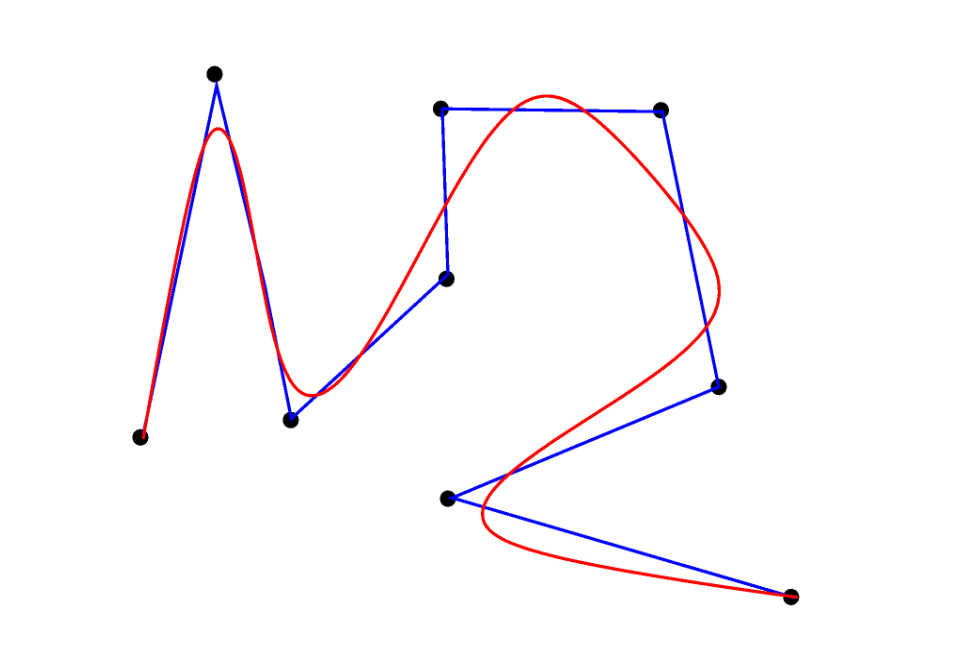
\includegraphics[width=10cm]{./img/bezier}
     \caption{From \cite{botta}. An example of B\'{e}zier curve: black points are the control point of the curve; blue lines simply connect with straight segments the control points; red line is the resulting B\'{e}zier curve.}
   \label{fig:bezier}
  \end{figure}
In addition, the authors compare two different methods to evaluate the evolved racing line; the first one is based on testing the evolved racing lines in a racing simulator; the second one consists of estimating the performance of a racing line through a computational model.
The former consists in making a TORCS predefined controller follow a determined trajectory. Then, a fitness function is computed as the lap-time achieved during the best lap. While this approach does not require any previous domain knowledge, as the fitness is the result of simulation, it is also rather expensive in computational terms as it requires a full simulation. 
On the contrary, the latter relies on a computational model which provides an estimate of the lap-time
that could be achieved following the racing line to evaluate. In particular, as soon as an estimate of the lap-time is available, the fitness function is computed as in the simulation-based method. This way, the computation is generally significantly less expensive than the simulation-based evaluation. As a drawback, a previous domain knowledge is required in order to create a model able to estimate the speed that can be reached in each point of the racing line. Moreover, the accuracy of the estimation depends on the precision of the model itself.

Another approach has been proposed in \cite{ahura}, where the authors implemented a controller called Ahura for TORCS based on heuristics.
The controller uses five modules: 
\begin{itemize}
\item Steer controller: This module uses the estimated angle
of the turn in front and the vacant distance in front to determine the steer angle. The module can control how smooth or sharp the vehicle is going to turn.
The main idea behind the calculation of the steer angle is to find the proximity sensor that has the maximum empty space in front (called the base sensor). The angle of the base sensor, together with some other auxiliary proximity sensors (as shown in Figure~\ref{fig:ahura-steer}), is then used to set the angle of the steer.
\begin{figure}
 \centering
  \captionsetup{width=10cm}
  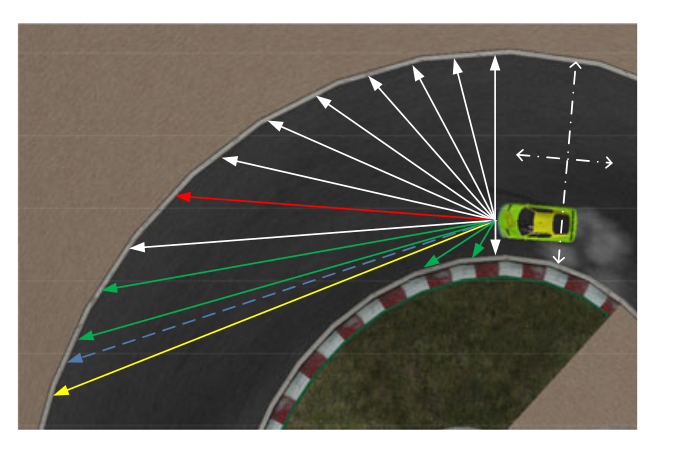
\includegraphics[width=10cm]{./img/ahura-steer}
  \caption{From \cite{ahura}. Red vector, the yellow vector, green vectors, and the blue vector represent the zero sensor, the base sensor, auxiliary sensors, and the final angle to take the turn, respectively.}
   \label{fig:ahura-steer}
\end{figure}
\item Speed controller: The aim of the speed controller is to determine the speed of the vehicle according to the current situation without considering opponents. This decision then is translated to the acceleration/breaking pedals. This module uses the estimated turn angle together with the vacant distance in front to decide the safe speed.
The target speed is mapped with a nonlinear function to values of acceleration and brake. Then, it is necessary to make sure that these values are applied in an appropriate way.  During the brake, the spin of the wheels might become smaller than the speed of the vehicle: that means that the wheels are slipping. Also, during the acceleration, the spin of the wheels might increase more than the speed of the vehicle: that means the vehicle is in traction. The ABS and ASR technologies solve these issues through keeping the speed of the spinning wheels and the speed of vehicle as close as possible.
Moreover, a gearing system is implemented, based on the minimum and maximum values of the rpm for each gear;
\item Opponent manager: This module creates a map of opponents around and finds the vacant slot to overtake. This action may entail modification of the speed and steer calculated by the speed and steer controller modules.
Ahura’s opponent manager contains two modules, steer reviser and speed reviser, that are responsible to revise steer and speed for overtaking. The information about opponents provided by opponent's sensors contain their distance and angle from the current position of the vehicle. This means that the position of opponents is provided in a polar coordinates system with the center of the measuring the vehicle. Ahura builds a spatial map of the position of opponents, which is used to revise steer and speed of the vehicle for overtaking purposes;
\item Dynamic adjuster: This module uses the mechanical specifications of the track (friction, bumps) as well as recorded difficulties the controller has experienced during the earlier laps and adjusts the current driving style.
The dynamics parameters are estimated using an optimization-based approach to find the best values so that Ahura can drive a specific bot in TORCS. There are 23 parameters in Ahura that need to be determined: eight parameters for the steer controller, ten parameters for the speed controller, five parameters for the opponent manager.
They were determined by using the optimization algorithm CMA-ES \cite{cmaes}, which has a good performance in continuous space, works with nonlinear systems, no constraint handling technique is required, and it is appropriate for nonseparable search spaces;
\item Stuck manager: This module controls the vehicle when it is out of the track or it has stuck somewhere.
The calculated parameters for the speed and steer controllers need to be revised based on the specifications of the track. The reason is that the parameters have been set for a limited number of tracks while new tracks might have different specifications. The main characteristics of tracks that may affect the best choice for parameters are friction, width, and bumps. Also, Ahura is able to handle stuck situation. In fact, if Ahura recognizes that the car is off the track, it reduces the maximum value of the acceleration pedal to prevent too much traction. It finds the correct direction first and tries to get back to the track. If it detects that the car is not moving, the gear is changed to -1 (rear gear) and the steer is adjusted accordingly to repair the direction of movement.
\end{itemize}


Existing advanced control based attempts to minimum-time driving usually provide only offline open-loop solutions.
In \cite{mpc}, the authors experimentally compared different time-optimal nonlinear MPC \cite{mpc_orig} formulations based on least squares objectives with an economic cost function in a real-time setup of small-scale model race cars, with the help of ACADO simulation toolkit from MATLAB \cite{acado}.
MPC, standing for Model Predictive Control is a multivariable control algorithm that uses an internal dynamic model of the process, a cost function over the receding horizon and an optimization algorithm minimizing the cost function using the control input.
The tight real-time bounds imposed on computational times make it necessary to reformulate the problem so as to allow for the use of efficient algorithms. To this end, they employed a nonlinear bicycle model \cite{bycicle} (see Figure~\ref{fig:bycicle}) in a reformulation to spatial coordinates and proposed an infeasible-time-tracking objective for the best practical results. In the literature, bycicle models are often adopted because, compared to higher fidelity vehicle models, system identification is easier, being there only two parameters to identify, $l_f$ and $l_r$.
For an approximate solution of the time-optimal driving problem, the aim is to minimize the time required for the race car to reach the end of the fixed-length spatial prediction horizon. For prediction horizons which tend to infinity this objective tends to the goal of driving time-optimally. As a consequence, long horizons are expected to yield a good approximation of the original problem in practice.
In the author's formulation, by providing a suffciently small (i.e., infeasible) "target time" \(T_{ref}\) they can have an approximate time-optimal MPC formulation in least-squares form. The performance of the car with this formulation is shown in Figure~\ref{fig:mpc-comparison} for several laps, where it can be seen that the cost
function allows the car to deviate from the centerline in order to minimize the time tracking error.
The real-world experiments showed that this approach has potential, but the bicycle model proved insufficient at high velocities due to slip effects not being modelled.
\begin{figure}
 \centering
  \captionsetup{width=10cm}
  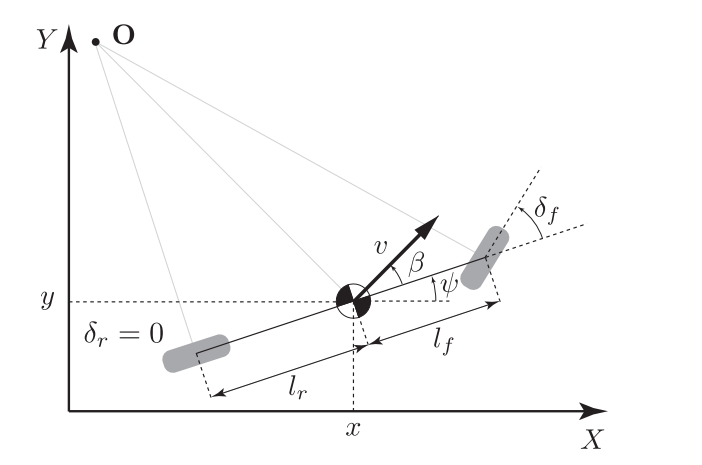
\includegraphics[width=10cm]{./img/bycicle}
  \caption{From \cite{bycicle}. Kinematic Bicycle Model: $x$ and $y$ are the coordinates of the center of mass in an inertial frame ($X$, $Y$). \(\psi\) is the inertial heading and $v$ is the speed of the vehicle. $l_f$ and $l_r$ represent the distance from the center of the mass of the vehicle to the front and rear axles, respectively. $\beta$ is the angle of the current velocity of the center of mass with respect to the longitudinal axis of the car. $\delta_f$ and $\delta_r$ are respectively the front and rear steering. Since in most vehicles the rear wheels cannot be steered, tipically $\delta_r$ is assumed equal to $0$.}
  \label{fig:bycicle}
\end{figure}
\begin{figure}
 \centering
  \captionsetup{width=10cm}
  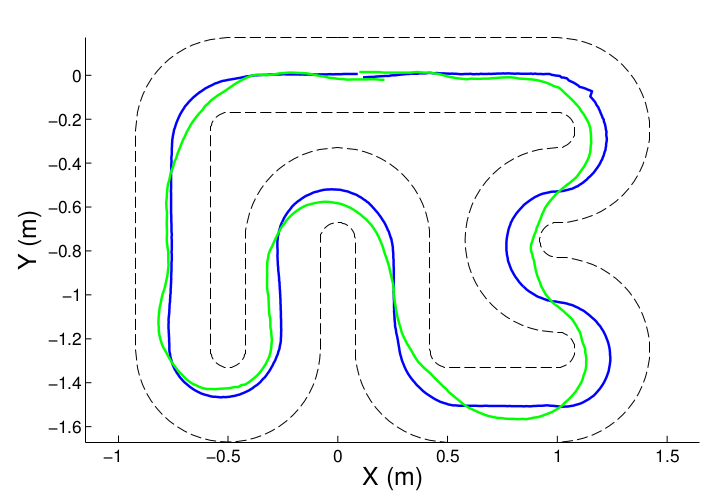
\includegraphics[width=10cm]{./img/mpc-comparison}
  \caption{From \cite{mpc}. Comparison of the performance of trajectory tracking and time-optimal driving on the experimental setup.}
	 \label{fig:mpc-comparison}
\end{figure}

\subsection{Reinforcement Learning in Racing Videogames}

With the evolution of technologies and algorithms, the focus has been shifting towards reinforcement learning and, in general, data-driven algorithms, which are achieving promising results in many applications, including autonomous driving and racing. 

In \cite{formularl} the authors tackle the problem by exploring different formulations of the DDPG algorithm \cite{ddpg} in TORCS.
Here, telemetry data are used in order to make an agent learn to drive and outperform the standard bots included in the simulator.
To achieve that, they provide the critic network of DDPG with a Long Short Term Memory \cite{lstm}, making the network recurrent, and enabling the agent to exploit the knowledge of the past. To this end, they also make the algorithm consider a window of multiple states and multiple reward instead of single ones.
While in the standard algorithm a one-step target is used for updating the critic function, they adopt a multi-step targets strategy, which incorporate the next $n$ rewards obtained along the trajectory starting from state $s_t$ and following a policy close to the current policy \(\pi\) at time step $t$.
Concerning the multiple states strategy, called Window sampling, the intuition is that in partially observable environments, accessing a single state does not reveal the full underlying state of the environment at each time step. Window sampling provides the agent additional information by feeding a window of the last $w$ states to the actor and the critic network.
Finally, they substitute the uniform distribution used by DDPG to sample the transition from the replay buffer with a Prioritized Experience Replay, which attempts to make learning more efficient by sampling more frequently transitions that are more important for learning.
Their study was split in three parts, by training three different models, in order to enhance the generalization capability. The first one uses a simple track and trained for $500$ episodes. The learned model was tested without exploration on the same track and the results were used to select the hyperparameters for each of the algorithms used. In the second one the algorithm has been tested on a technically more complex track, while in the last part they evaluated the impact of adding future information of the track by adding a look ahead curvature and training in all three tracks.


\subsection{Imitation Learning in Videogames}

A promising approach in building human-like artificial players is what is commonly known as Imitation Learning \cite{imit1, imit2, il}, or Learning from Demonstration (LfD) \cite{lfd}, which consists in integrating some human expertise in the algorithm.
Some of the techniques employed in IL can be employed in RL algorithms to accelerate the learning process.


A popular algorithm called DAGGER \cite{dagger} provides an easy way for incorporating human experience. However, a human expert should always be available to provide feedback which is unrealistc in practice. 

Presented in \cite{dqlfd}, Deep Q-learning from Demonstrations (DQfD) vastly accelerates DQN by pretraining an initial behavior network, and also introducing a supervised loss and a L2 regularization loss when training the target network.

In \cite{drlhp} the authors considered rewards computed by a predictor trained with human feedback rather than from  interactions with the environment. This method separates the goal learning from the behavior learning by training a reward predictor with non-expert human preferences, and the behavior of the agent is improved accordingly.

\subsection{Imitation Learning in Racing Videogames}

Togelius and colleagues focused on the learning of a specific driving style using a simple 2D car simulator \cite{imit3}, \cite{imit4} and TORCS \cite{imit5}. In \cite{imit3}, the authors applied supervised learning (more precisely, neural networks and k-nearest neighbor \cite{knn}) to model driving styles directly, that is, by building models that could accurately predict the player actions based on the current game state. However, direct modeling resulted limited performance, accordingly, they moved to indirect modeling and used a genetic algorithm to evolve a controller with a driving style similar to a target human player. In \cite{imit4}, the approach based on indirect modeling was improved by using a different fitness function while later, in \cite{imit5}, it was extended by introducing a multi-objective evolutionary algorithm to evolve controllers which could be both robust (in that, they never run out of the track) and could demonstrate a driving style similar to one recorded from a user (in that, they accurately predict the user actions).


In  \cite{cardamone}, Cardamone, Loiacono and Lanzi applied supervised learning to develop car controllers in TORCS from the logs collected from other driver, and developed controllers capable of driving in non-trivial tracks reaching a performance that is in some cases 15\% lower than that of the fastest bot available in
the simulator (a good result if considered that supervised learning approaches generally yield poor performances).
They considered two representations of the current state of the car:
\begin{itemize}
\item The first sensory representation is based on a rangefinder inputs usually employed in simulated car racing competitions.
The rangefinder casts an array of beams, with a range of 100m, around the car and returns the distance from the car to the track edge;
\item  A high-level, qualitative, representation involving basic lookahead information about the track in front of the car, based on a  novel sensor model, called lookahead sensor (see Figure~\ref{fig:cardamone2}). This representation is inspired by the behavior of human drivers whose decisions are usually based on high-level information about the current speed and trajectory and on the shape for the track ahead. 
For this purpose, the next $h$ meters of the track ahead are considered and divided into segments of the same length, and the lookahead sensor returns the bending radius for each segment: a rectilinear segment corresponds to a $0$; a positive radius corresponds to a right turn; while a negative radius corresponds to a left turn. 
\end{itemize} 

\begin{figure}
 \centering
  \captionsetup{width=10cm}
  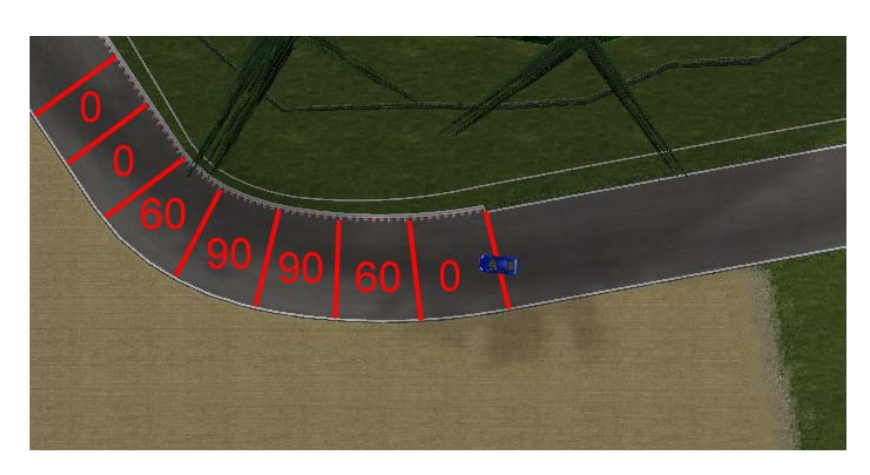
\includegraphics[width=10cm]{./img/cardamone2}
  \caption{From \cite{cardamone}. Lookahead Sensor.}
   \label{fig:cardamone2}
\end{figure}
\begin{figure}
 \centering
  \captionsetup{width=10cm}
  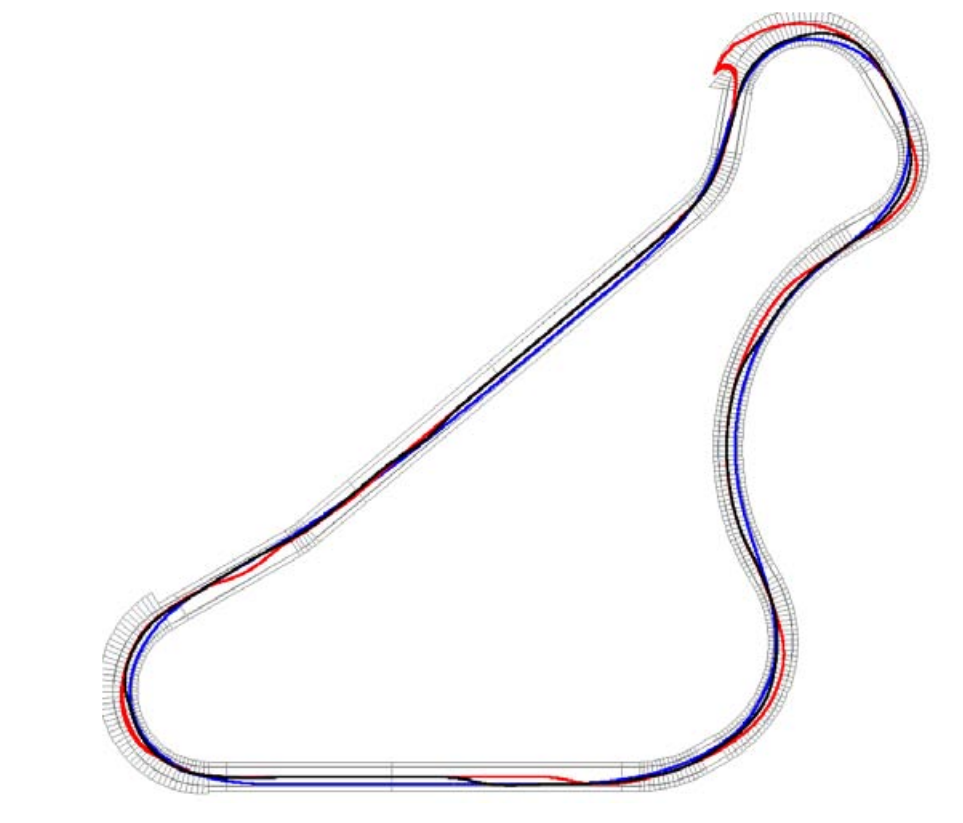
\includegraphics[width=10cm]{./img/cardamone}
  \caption{From \cite{cardamone}. Trajectories comparison in track G-track-1: bot Inferno (blue line), 8 segments lookahead (red line), 16 segments lookahead (black line).}
  \label{fig:cardamone}
\end{figure}

Regarding the control phase, rather then acting on steer, throttle and break pedal, they propose  to control the car at a higher level. They try to learn the trajectories and the speeds along the track rather than low level commands.
In other words, instead of predicting the typical low-level actions on the car actuators available in TORCS, their approach is to predict a target speed and the car position with respect to the track axis.
A trajectory can be represented as the distance from the track axis in each segment of the track. So the output variables of the controller are the speed and the axis distance in the current segment.
The control is realized by means of three simple algorithms:
\begin{itemize}
\item Algorithm 1 computes the steer value: it describes the simple policy that controls the steering command to reach the target distance from the track axis. First, the wheel is aligned to the car axis and then a correction is applied to reduce the error;
\item Algorithms 2 computes the acceleration value;
\item Algorithms 3 computes the brake value. 
Algorithms 2 and 3 work this way: simply accelerate at full speed when the current speed is low and brake when is too high. 
\end{itemize}
A soft transition is finally applied between brake and accelerator when the actual speed is near to the target speed. This way, switching from full acceleration to full brake is avoided, resulting in no fluctuations around the target speed.

 
Finally, as concerns the learning phase, they considered two supervised learning methods, k-nearest neighbor classifiers \cite{knn} and multi-layer neural networks \cite{neat}, and applied them to compute a model mapping input sensors to actions which could imitate the behavior of an observed driver.
The model was then deployed to a driver controller that would map the high-level actions predicted by the models to low-level actions of the usual TORCS effectors
using the algorithms discussed in the previous section.

\textbf{KNN.} k-nearest neighbour does not involve any training in that the collected data represent the model. Accordingly, it has been directly applied during the evaluation, i.e. during a race using TORCS. At each game tic, the logged data are searched to find the k most similar instances to the current sensory input using either the typical rangefinder representation or the new lookahead representation. The k similar instances are selected and the corresponding outputs variable are averaged to predict the target value. The similarity measure used is simply the Manhattan distance among instances;
\textbf{Neural Networks.} To avoid the issue of selecting a particular neural network structure, they applied Neuroevolution with Augmenting Topology (NEAT) \cite{neat} which applies a genetic algorithm to evolve both the weights and the topology of a neural network. They evolved two separate neural networks, one to predict the target speed and one to predict the target position for a given input configuration. The fitness was defined as the prediction error computed as the total sum of the absolute error between the true value and the predicted value, for each instance in the training data. 
Their experiment consisted in running the Inferno bot on three tracks: G-track-1, a simple track; Wheel-1, a more difficult track with many fast turns; and Aalborg, a difficult track with many slow sharp turns. They logged the data from the rangefinders and from the lookahead sensors, together with the car distance from the track axis and the car speed which we use
as outputs.
The learned trajectories are shown in Figure~\ref{fig:cardamone}.




This paper \cite{cinesi} aims at improving the achievements of DQfD \cite{dqlfd} in integrating reinforcement learning with human demonstrations using TORCS.
Their goal is to bring experts demonstrations together with reinforcement learning, try to let the agent learn an appropriate policy by interacting with the environment on itself, and learn from expert’s demonstrations at the same time.
Their contribute develops in three parts:
\begin{itemize}
\item They shift from the discrete action domain considered in \cite{dqlfd} to a continuous action domain.
In order to determine the similarity between actions, they approximately evaluate the two considered actions by their mean squared error.  As DQN uses a greedy way to find the optimal policy, and the actions are finite discrete values, it is easy to calculate the supervised error for DQfD. However, in continuous action domain, the greedy policy is inapplicable, so they try to use the output of actor network directly for supervision. They combine a supervised loss with the original TD-loss to update the parameters of the critic network, and control the weighting between the losses by a given parameter;
\item They adjust the Experience Replay of DQN and DDPG by constructing an integrated replay buffer, which improves DDPG stability.  In DQN, the authors use a replay buffer to store the transitions generated by interacting with the environment, and randomly sample batches for training. In DQfD, two replay buffers are employed to store the self-generated data and demonstrator’s data respectively. Training data is sampled from these two buffers by a certain proportion. In this paper, the authors added another buffer to store the self-generated training data with good performances. 
For the initlia episodes, which usually do not contain enough good data, they instead use another buffer to collect the best transitions in every training episode, and substitute for the good performance buffer temporally. 
Their claim is that this procedure may improve the performance and stability of training;
\item  They attempt to learn human preferences without contradicting to the overall target of the task. Most RL methods have only an overall goal, but they do not consider the human behavior in realizing the goal, which can be reflected from the slightly differences between human personal preferences in completing the same task. They tackle this problem by recording demonstrations with human preferences and define specific optimization objectives to ensure the consistence with human preferences. To do that, they use demonstration data as the critic network’s inputs. The actor network yields an action, which must be similar enough with the demonstrator’s one. Meanwhile, this action needs to satisfy the Bellman Equation and to yield higher rewards when interacting with the environment. So, they use a combined loss to update the critic network’s parameters.
\end{itemize}
Their claim is that their method not only masters the preferences in choosing the lane, but also outperforms human expert demonstration in average reward.



Our work takes place in this context of imitation learning integrated with reinforcement learning applied to autonomous driving in TORCS without using sensory information. In the next section, we illustrate the software architecture and thereafter we describe techniques we used. 
